\documentclass[12pt]{amsart}
\usepackage{geometry}                % See geometry.pdf to learn the layout options. There are lots.
\geometry{letterpaper}                   % ... or a4paper or a5paper or ... 
%\geometry{landscape}                % Activate for for rotated page geometry
%\usepackage[parfill]{parskip}    % Activate to begin paragraphs with an empty line rather than an indent
\usepackage{graphicx}
\usepackage{amssymb}
\usepackage{epstopdf}
\usepackage{hyperref}

\hypersetup{
    colorlinks=true,
    linkcolor=blue,
    filecolor=magenta,      
    urlcolor=cyan,
}
 
\urlstyle{same}

\DeclareGraphicsRule{.tif}{png}{.png}{`convert #1 `dirname #1`/`basename #1 .tif`.png}

\title{Correcting Presidential Comparisons of Employment Growth}
\author{Nathaniel Bechhofer}
%\date{}                                           % Activate to display a given date or no date

\begin{document}
\maketitle

\section*{Background}
% krugman.blogs.nytimes.com/2015/12/27/obama-the-job-killer/
When comparing the performance of presidents, an obvious choice is employment growth. In fact, political science models often use employment situations to predict how well an incumbent president will do when attempting to obtain a second term. However, the employment picture in the United States at any time cannot be summarized with one number. One standard method to use is changes in private-sector employment, as the president would presumably be unable to directly influence the employment decisions of private companies. Nobel laureate Paul Krugman used this to compare the relative performance of the 43rd president, George W. Bush, and his successor, Barack Obama. His post for the New York Times can be found \href{http://krugman.blogs.nytimes.com/2015/12/27/obama-the-job-killer/}{here}.

\section*{The original figure}

\begin{figure}[!htbp]
\begin{center}
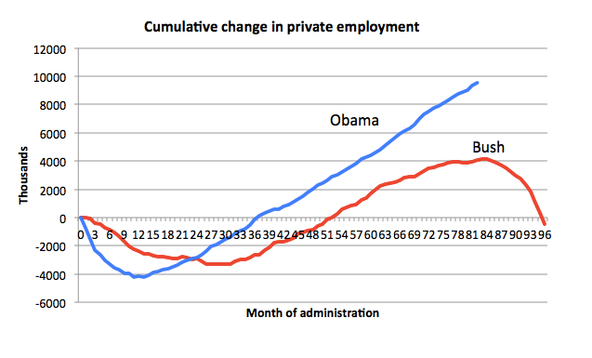
\includegraphics[width=\textwidth]{Original.png}
\caption{The figure used in Krugman's original blogpost.}
\label{orig}
\end{center}
\end{figure}

The comparison Krugman made used the graph shown in Figure \ref{orig}, which could use some improvement to help readers draw relevant conclusions. For one thing, the tick labels are far too dense. The gridlines are not easy to make out, and the lack of vertical gridlines forces the reader to rely on their own brain to draw lines perpendicular to the x-axis. Furthermore, the comparisons made use absolute numbers, which are not very helpful when one is not intimately familiar with the numbers involved. The redesign presented below fixes these issues, but it also takes into account one more thing: how the age distribution of the US population shifted over time. Indeed, the aging of America's workforce is well known, and it would seem implausible that this would not affect employment variables. Therefore, an adjustment process is advisable.


\section*{Age-adjustment methodology}
The Bureau of Labor Statistics (BLS) has described a \href{http://www.bls.gov/opub/mlr/2002/09/art3full.pdf}{fairly standard age-adjustment procedure}, which is adopted here. We can first apply this procedure to the ratio of employment to population (EPOP).
To obtain an estimate of how the EPOP changes over time when accounting for age, we use the following formula:
\begin{equation*}
Y_t = \frac{\sum (r_t \times n_{\text{base}})}{\sum n_{\text{base}}}
\end{equation*}
where $r$ is the proportion of a particular age group employed and $n|{\text{base}}$ is the is number of people in the age group in the population for the year we choose as the base year for demographic comparison. 

In this case, I use the year 2000 for all data, so that both presidents will be subject to the same adjustment. Moreover, I use four different age groups: people between 16 and 19, people between 20 and 24, people between 25 and 54 (prime-age workers), and those at least 55. Though we would ideally have more precision, the approximation here works well because employment rates correlate very highly within these groups. 
%http://www.bls.gov/opub/mlr/2002/09/art3full.pdf

After calculating this adjusted EPOP (using eight different data series), I can then use the ratio of the adjusted EPOP and the given EPOP to make the employment numbers more meaningful. Multiplying this ratio by the original variable (presented without the seasonal adjustment used in Krugman's case) allows readers to track a variable which is not primarily driven by changes in the age distribution.



\section*{Presenting the Redesign}
\begin{figure}[!htbp]
\begin{center}
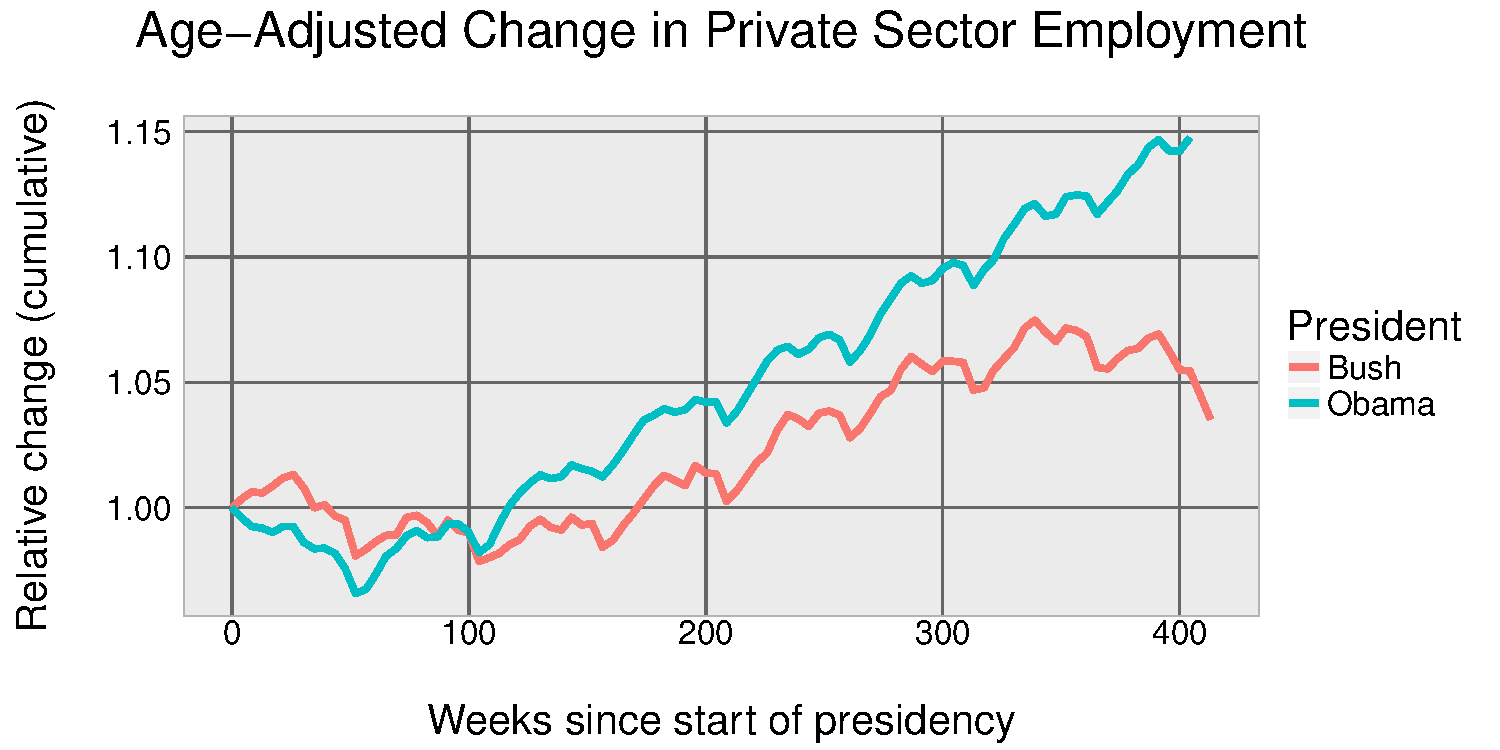
\includegraphics[width=\textwidth]{Main_plot.pdf}
\caption{An improved version of the graph.}
\label{improved}
\end{center}
\end{figure}

The new version, shown in Figure \ref{improved}, tells a very different story. Rather than showing a complete failure of the Bush presidency, it is apparent that there was genuine net improvement in private-sector employment over the whole eight years (when one has considered the effects of age). This does not negate the very real advantage of the Obama years; in fact, this makes it easier to see a consistently higher slope for \textbf{relative} change in the Obama years. The redesign can be used to strengthen the beliefs of a partisan of either side, but at least it tells a more accurate story, as the variable used is more suited to evaluating presidential performance (presidents can't do very much to affect the age distribution in their term). 

\end{document}  